\chapter{Khorabiè}
\label{ch:khorabie}
\index{dessert}
\index{cookies}
\index{dates}
\textit{Biscuits aux dattes}

Family member: Metzma Lucie

\marginnote[20pt]{\\
    \textbf{Makes 24+ cookies} \\
    Prep time: 2-3 hours \\
    Cook time: 12-15 minutes \\
    \vspace*{\baselineskip}

    1 cup vegetable oil \\
    1 cup milk \\
    250ml butter, melted (or unsalted margarine) \\
    1/2 packet of Crisco, melted \\
    3 tsp baking powder \\
    1 cup icing sugar \\
    6-6 1/2 cups flour \\
    1 kg dates, in puree (in a packet) \\
    Zest and juice of 1 orange \\
}

\begin{marginfigure}[20pt]
  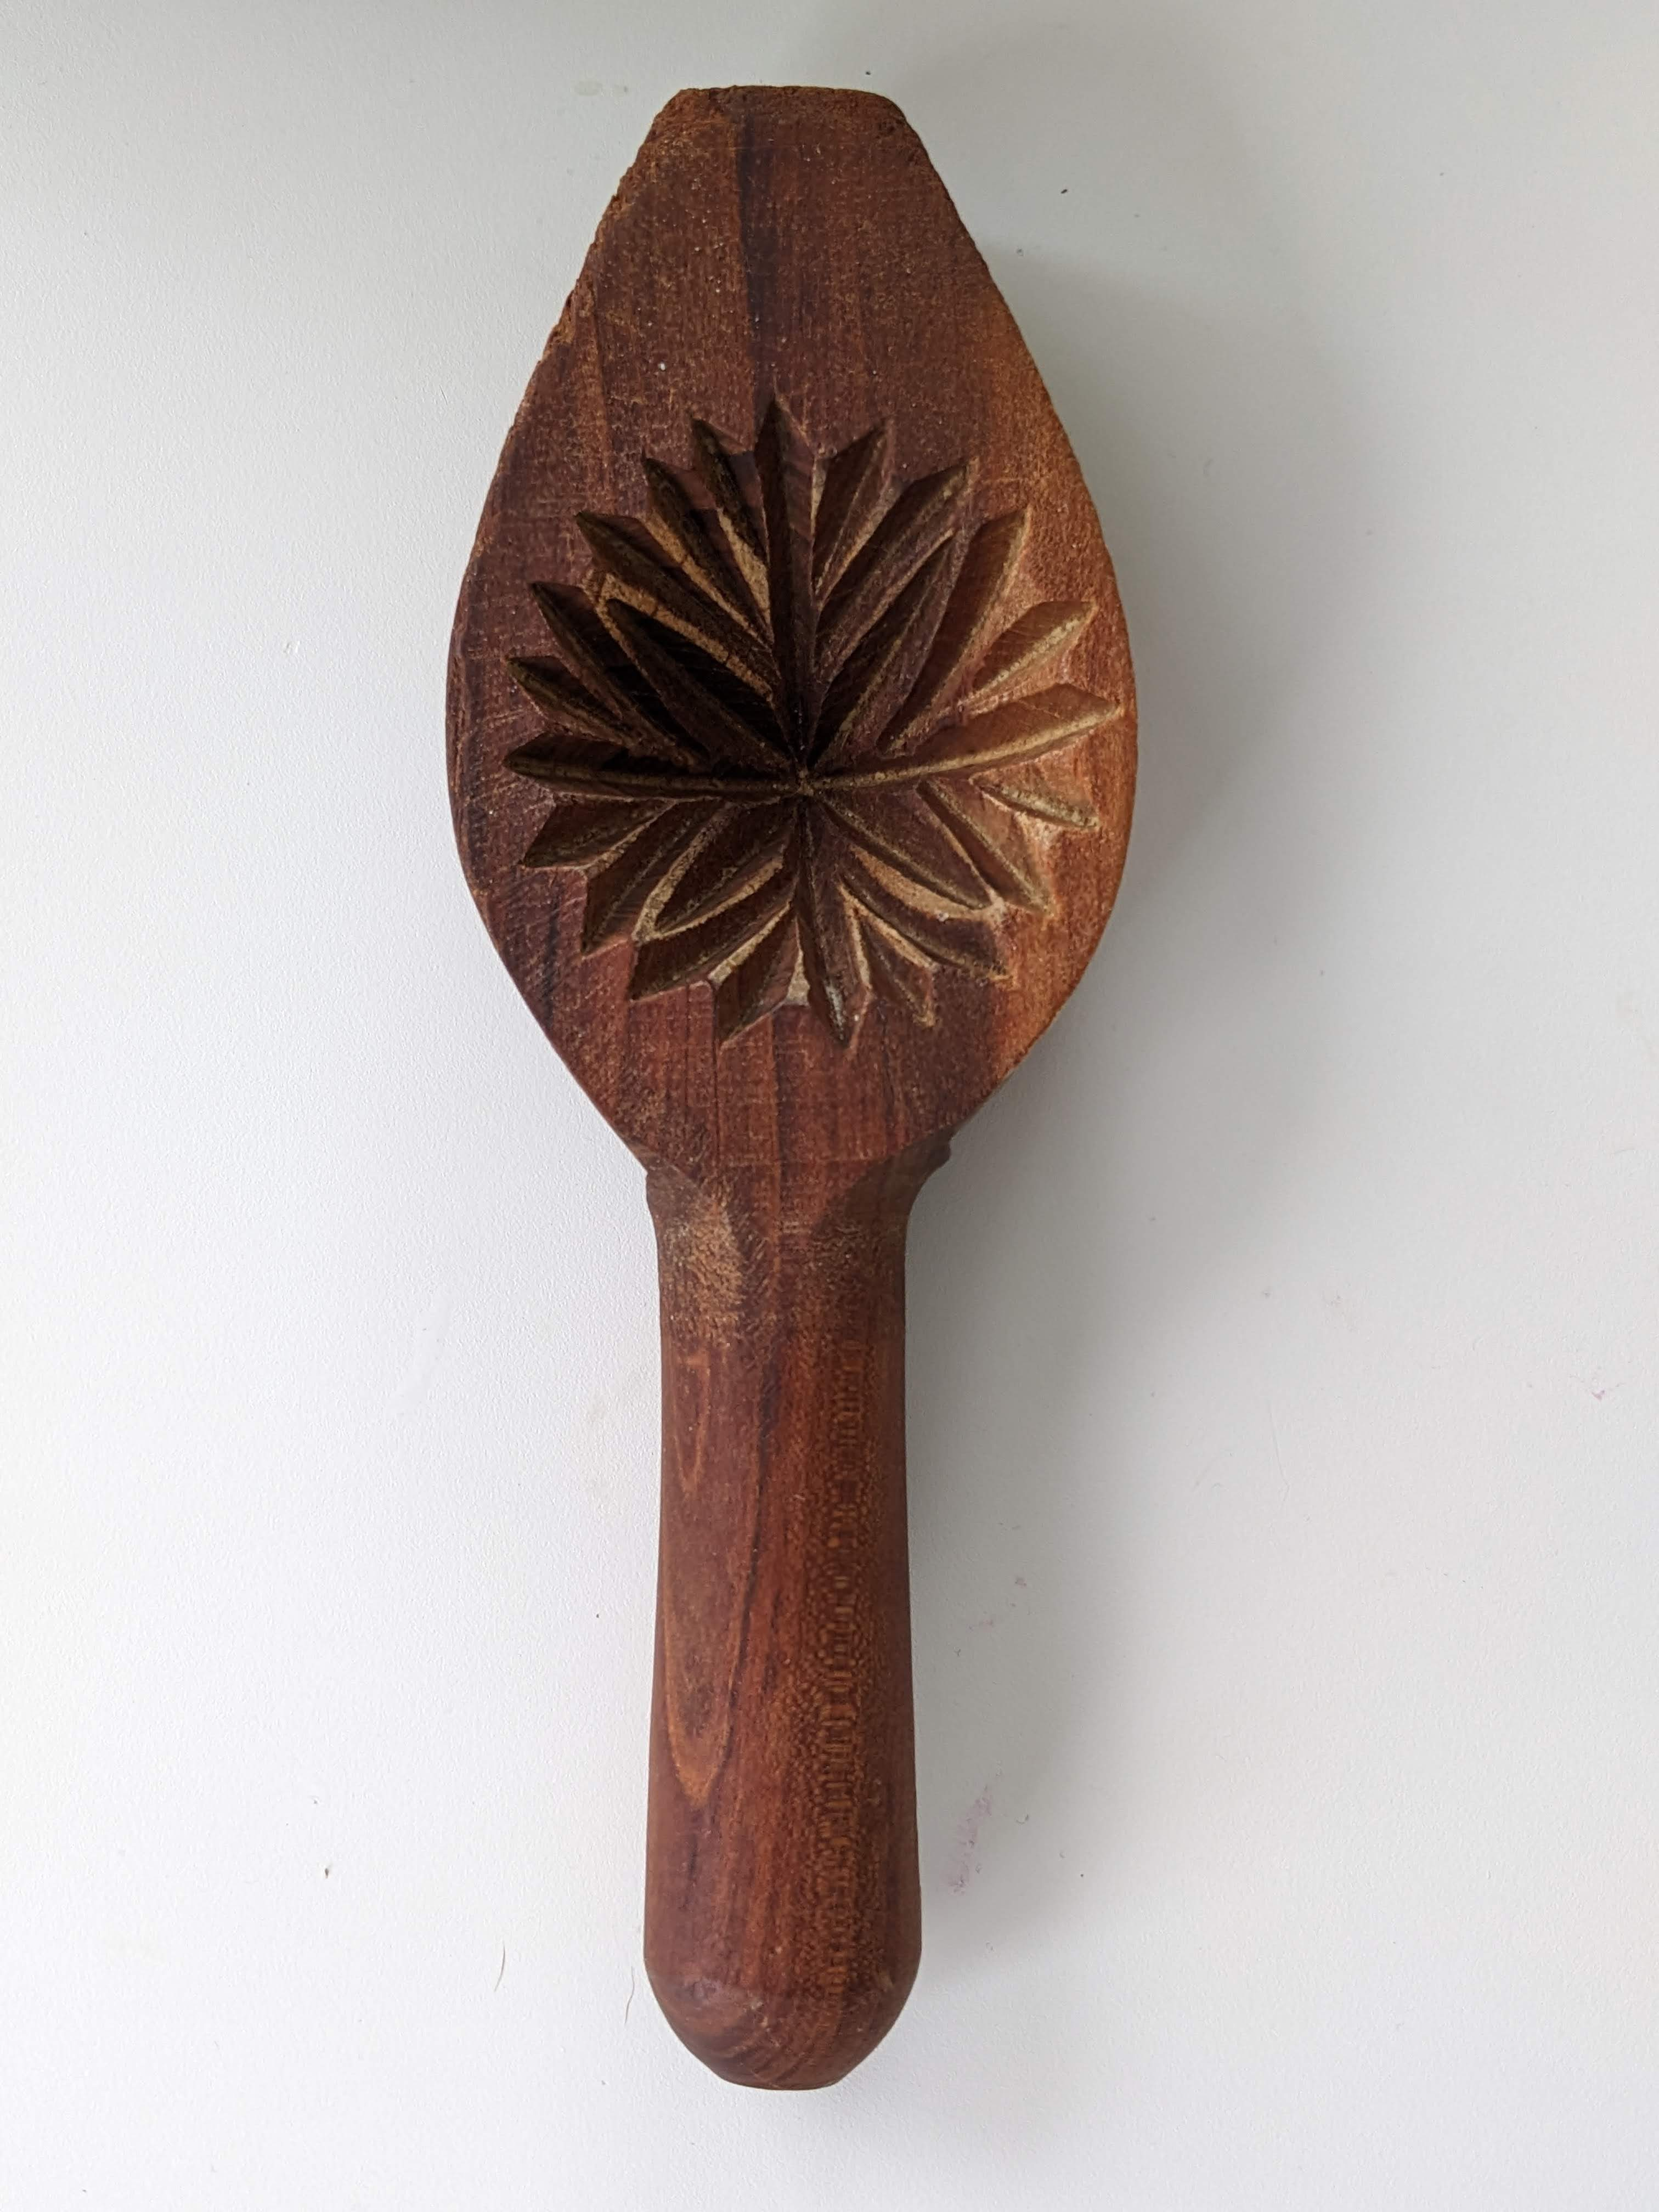
\includegraphics[width=60mm]{dermardiros/images/PXL_20240427_185332023.PORTRAIT.ORIGINAL.jpg}
  \caption{Khorabiè mold}
\end{marginfigure}[20pt]

% \newthought{}
% \bigskip

\begin{enumerate}
    \item In a bowl, mix the oil, milk, melted butter and melted Crisco.
    \item In another bowl, mix the baking powder, icing sugar and flour.
    \item Sift the dry ingredients onto the wet ingredients, then mix with hands until you form a dough. You can add more flour as needed to form a ball.
    \item In a small bowl, mix the dates with the orange zest and orange juice.
    \item Shape balls of dough, make a small well in the center and stuff with the date filling. Enclose the dates in the center with the dough. 
    \item Lightly flour the wooden khorabie mold and gently press the ball inside the mold to obtain a shape on one side.
    \item Place the shaped cookies onto a baking sheet and bake 12-15 minutes on the middle rack at 350\degree F until the tops have a golden color. 
    \item Let cool and sift some icing sugar on top. Enjoy with coffee or tea!
\end{enumerate}